\documentclass[dvipdfmx]{beamer}
\usepackage{tutorial}
\title{計算機実験 --- \\ スーパーコンピュータと計算物理}

\begin{document}

\lstset{language={C},basicstyle=\ttfamily\scriptsize,showspaces=false,rulecolor=\color[cmyk]{0, 0.29,0.84,0}}

\begin{frame}
  \titlepage
  \tableofcontents
\end{frame}

\section{スーパーコンピューターと計算物理}

\begin{frame}[t,fragile]{計算機の進化}
  \begin{itemize}
    \setlength{\itemsep}{1em}
  \item 計算機の性能は指数関数的に伸び続けている
    \begin{itemize}
    \item 1年で1.9倍 ⇒ 4年で10倍 ⇒ 過去70年間で100兆倍
    \item 世界初のスパコンCray-1 (1976年)の演算性能 約160MFlops
    \item iPhone6 (2014年)の演算性能 約900MFlops
    \item 2020年代初頭には、1EFlops (エクサフロップス)へ
    \end{itemize}
  \item 現代のスーパーコンピュータは全て
    \begin{itemize}
      \item 並列コンピュータ (CPU数 1,000〜100,000)
      \item マルチコア or メニーコア (CPUあたりのコア数 8 〜 1,000)
      \item 多層にわたる階層構造
      \item 演算に比べて、データを移動するコストの方が高い
    \end{itemize}
  \end{itemize}
\end{frame}

\section{バッチキューシステム}

\begin{frame}[t,fragile]{バッチキューシステム}
  \begin{itemize}
    \setlength{\itemsep}{1em}
  \item 実習用計算機 photon
    \begin{itemize}
    \item ログインノード(2CPU, 12コア)+計算ノード(64CPU, 256コア)からなる「クラスタワークステーション」(並列計算機の一種)
    \item 普段{\tt ssh}して作業しているのはログインノード
    \end{itemize}
  \item バッチーキューシステム
    \begin{itemize}
    \item 長い(大きな)計算は計算ノードを使う
    \item 多数の計算ノードの割り振りを手でやるのは非効率的
    \item バッチキューシステムを使って、「ジョブ」を投入する
    \end{itemize}
  \item 詳しい説明は「システム利用マニュアル」({\tt ssh}ログイン時に表示されるメッセージ参照)を見ること
  \item photon は卒業まで継続して利用可 (希望すれば大学院でも)
  \end{itemize}
\end{frame}

\section{並列計算とは}

\begin{frame}[t,fragile]{Richardson's Forecast Factory (1922)}
  \resizebox{.8\textwidth}{!}{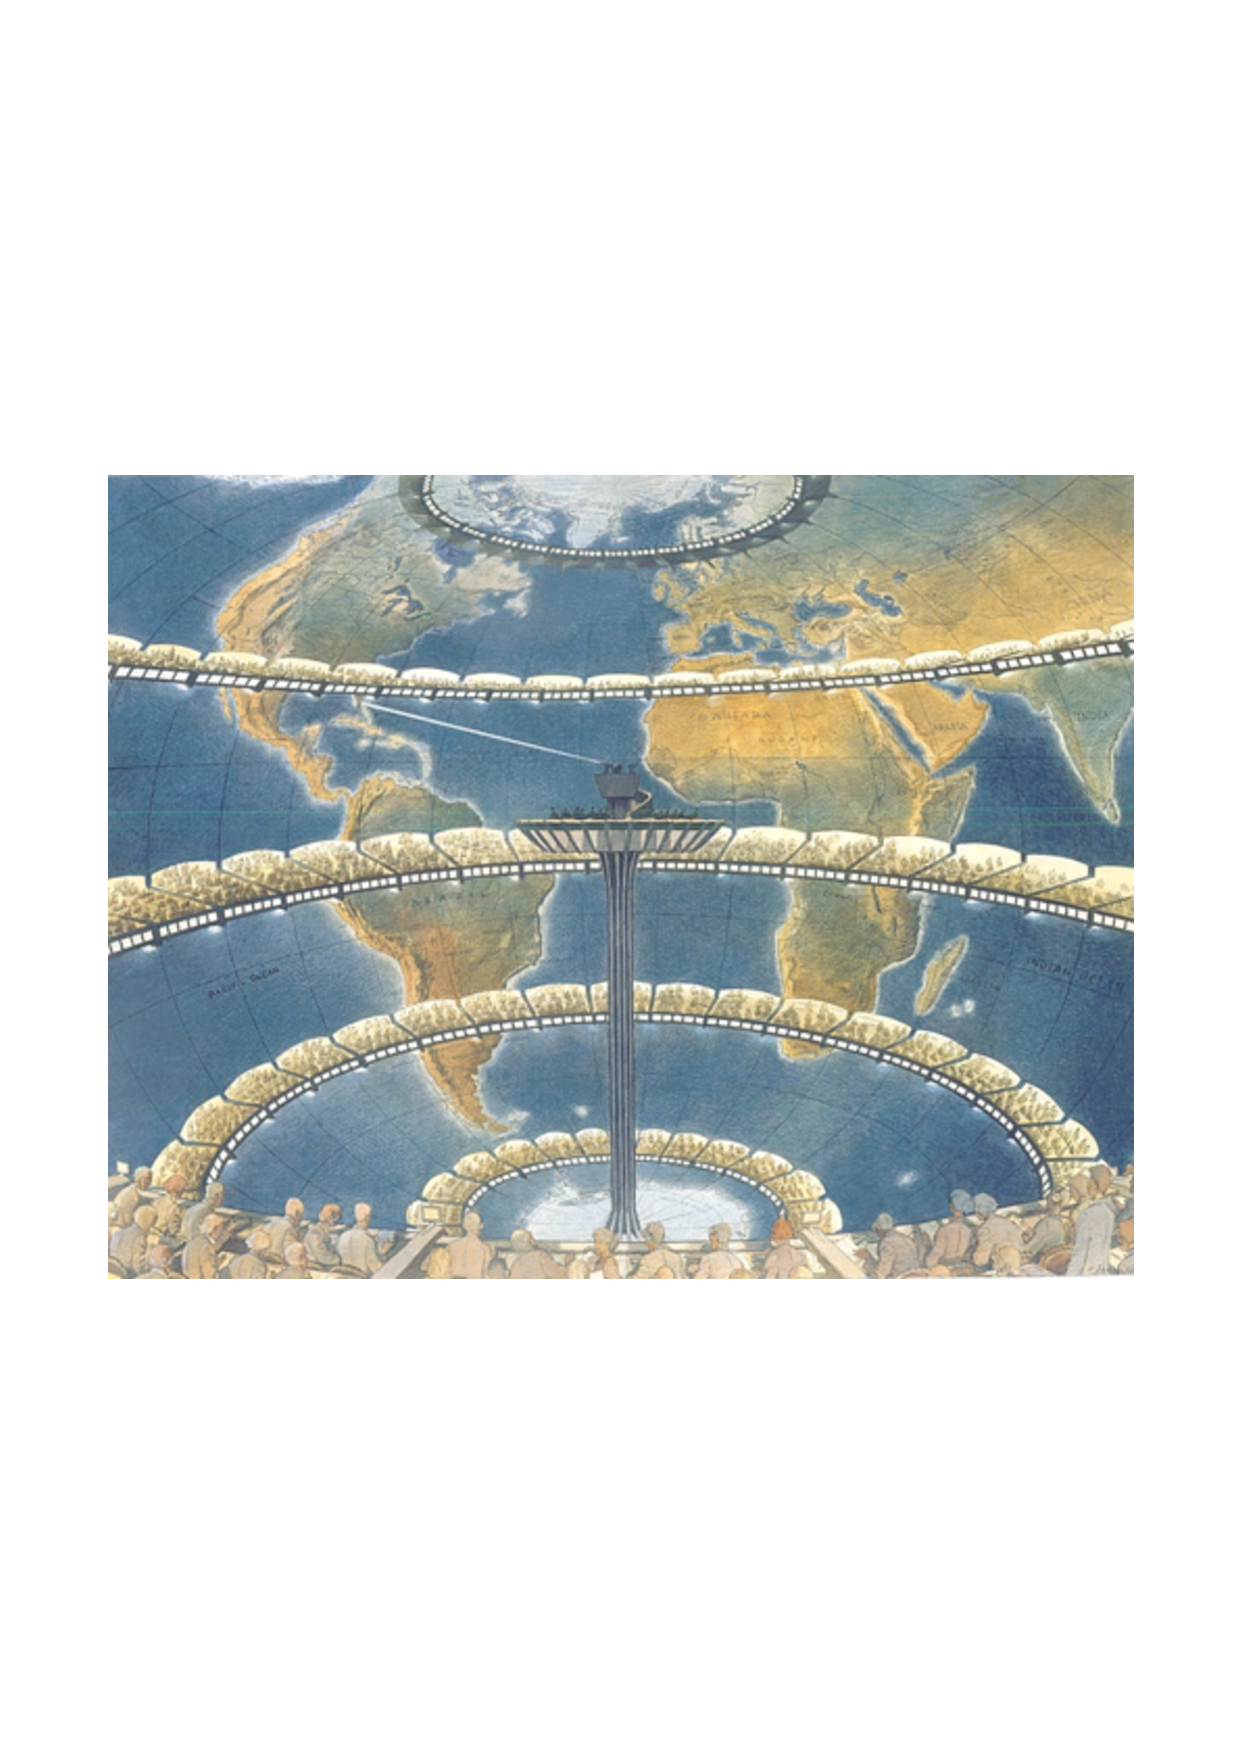
\includegraphics{image/SchuitenHD3.pdf}}
\end{frame}

\begin{frame}[t,fragile]{並列化とは何か}
  \begin{itemize}
    \setlength{\itemsep}{1em}
  \item 目的: シミュレーションをできる限り「短時間」で終了させる
    \begin{itemize}
      \item たとえ総CPU時間が伸びても「ターンアラウンド時間」を短かくしたい
      \item 一台のパソコンでは100年かかる計算を学位論文に間に合わせたい
      \item 今の100倍の精度の計算を同じ「実時間」で実行したい
    \end{itemize}
  \item 並列化とは
    \begin{enumerate}
    \item CPUの行なうべき仕事を複数の小さな仕事に分割
    \item それらを複数のCPUで同時実行
    \end{enumerate}
  \item うまく並列化を行なうために必要なこと
    \begin{enumerate}
    \item プログラムのどの部分をどのように並列化すればより効果的かを理解する
    \item 並列化を実装するにはどのようにプログラムを書けば良いかを理解する
    \end{enumerate}
  \end{itemize}
\end{frame}

\begin{frame}[t,fragile]{並列計算の原理}
  \begin{itemize}
    %\setlength{\itemsep}{1em}
  \item ノードは、互いに必要な情報を交換しながら、それぞれ異なる処理をしなければならない
  \item ノード毎に異なる指示(= プログラム)を与えるのは大変 (特にノード数が何万もの場合)
  \item 一つのプログラムでノード(ランクとも呼ばれる)毎に異なる指示を与えたい

    ⇒ SPMD (Single Program, Multiple Data streams)

    \resizebox{.9\textwidth}{!}{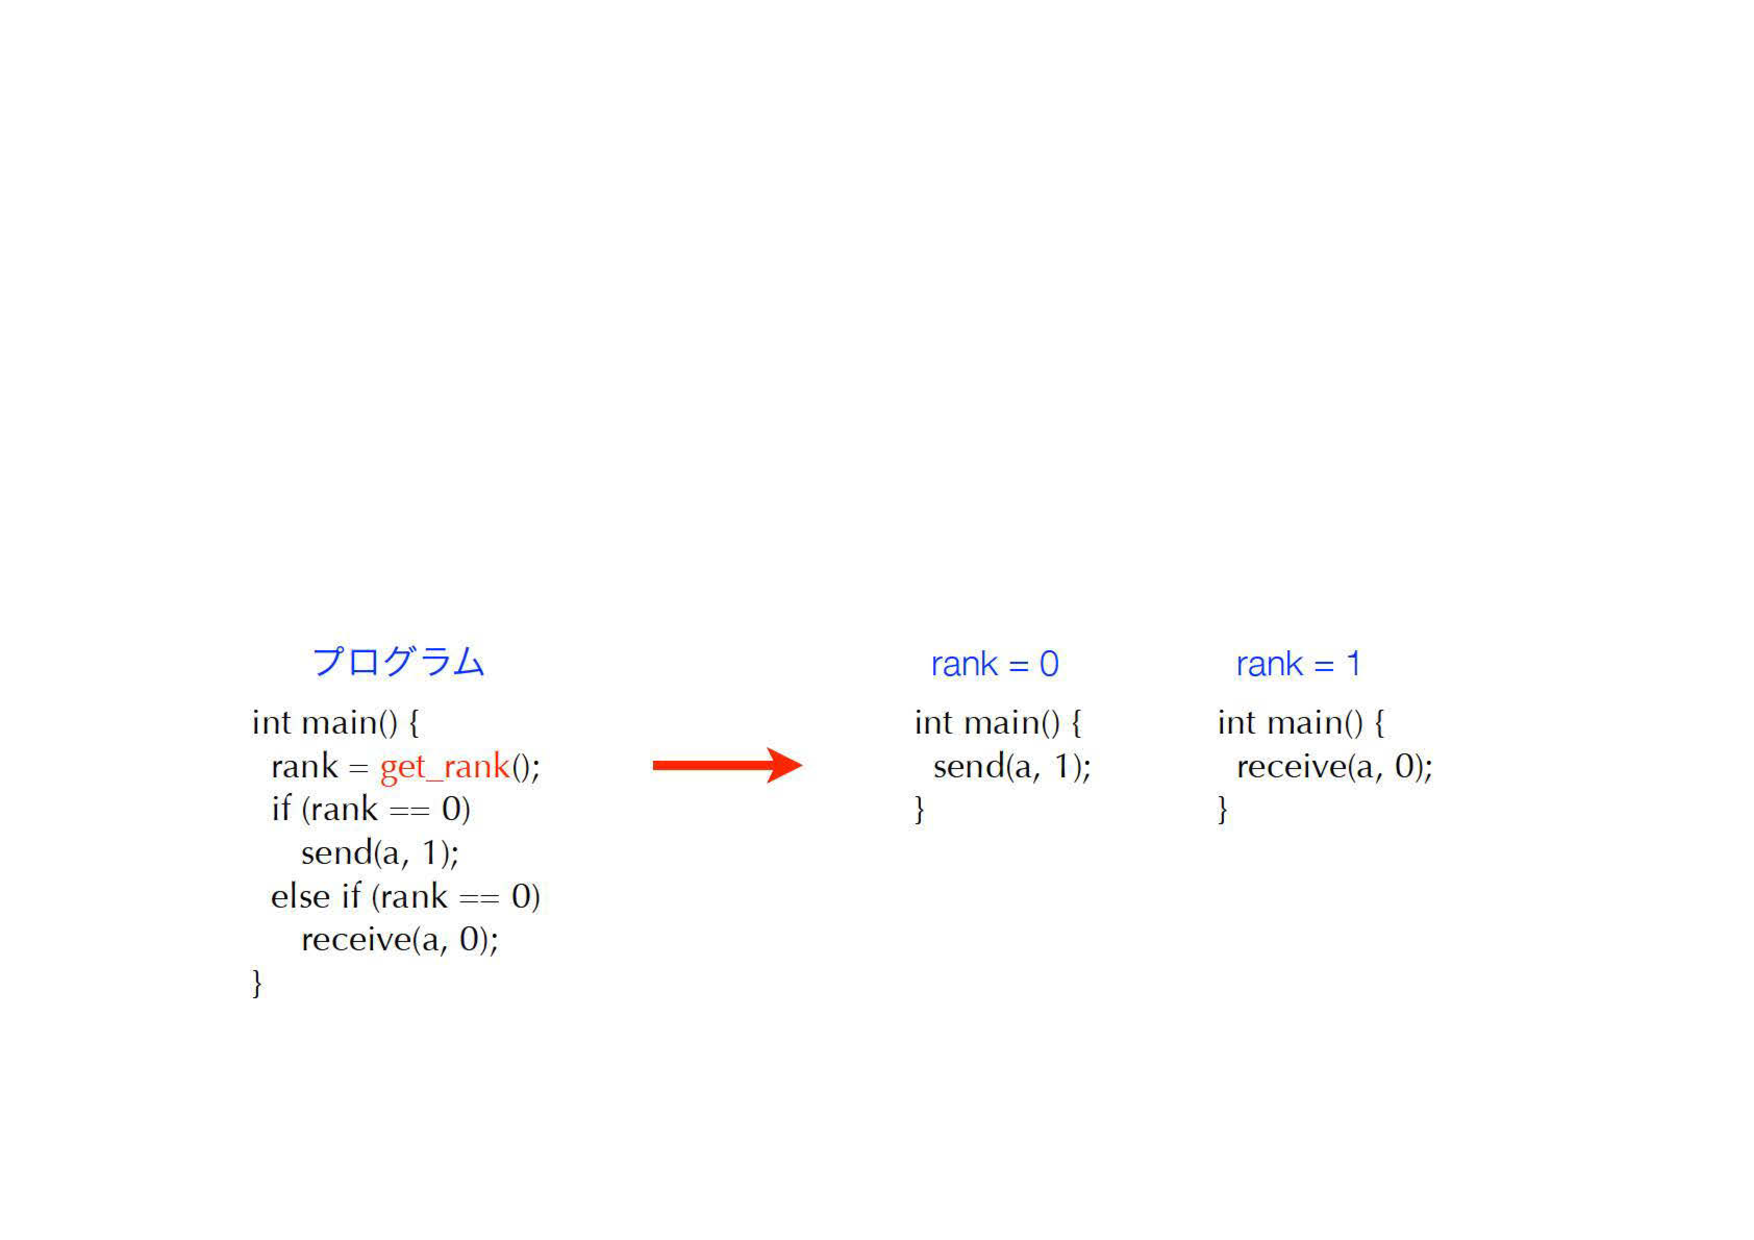
\includegraphics{image/spmd.pdf}}
  \end{itemize}
\end{frame}

\begin{frame}[t,fragile]{アムダール(Amdahl)の法則}
  \begin{itemize}
    \setlength{\itemsep}{1em}
  \item 並列化による全体の性能向上率
    \[
    P = \frac{1}{X+(1-X)/n}
    \]
    $X$: 並列化されていない部分の実行時間の割合, $n$: ノード数
  \item $X$を限りなく零にしないと高並列ではすぐに性能が頭打ちに
  \end{itemize}
  \vspace*{-0em}\hspace*{1em}\resizebox{0.5\textwidth}{!}{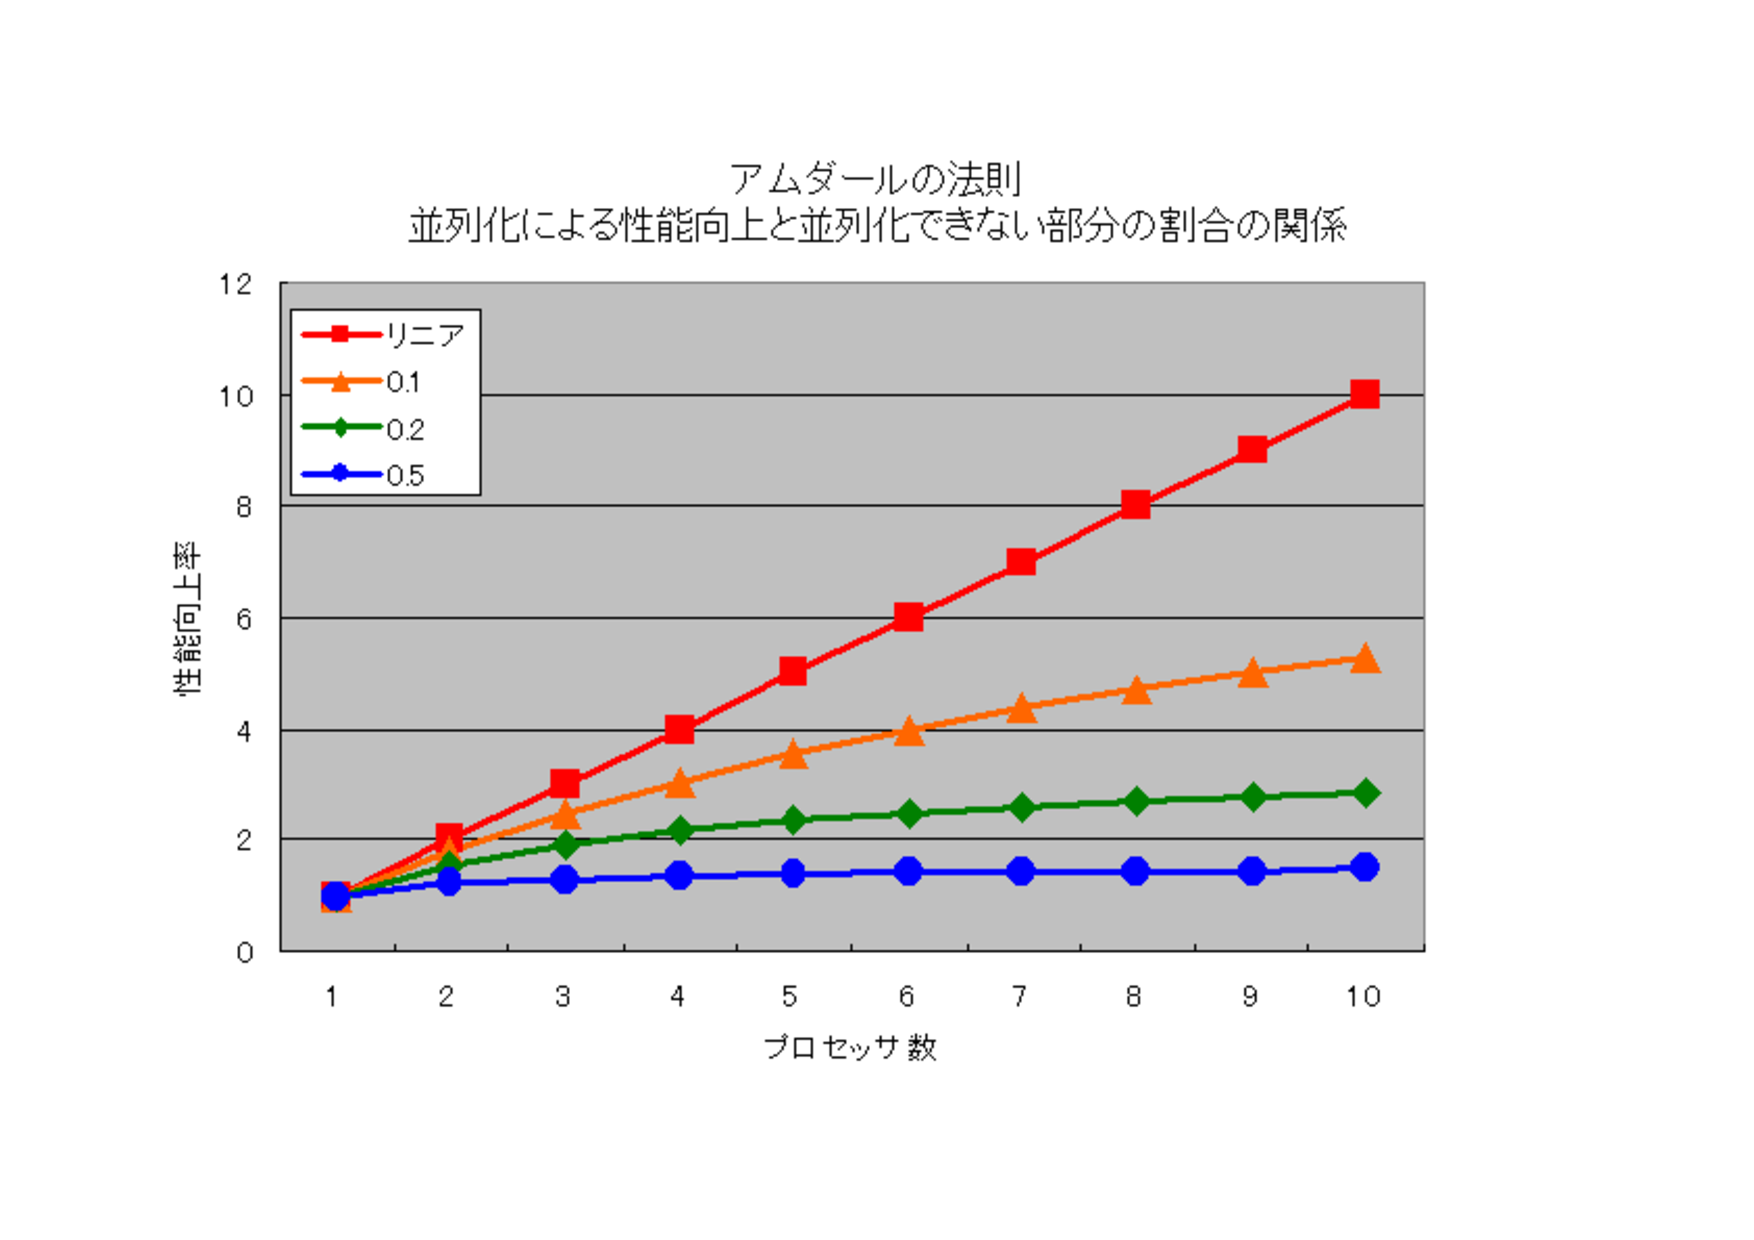
\includegraphics{image/Amdahl_law2.pdf}}
\end{frame}

\section{実習その3}

\begin{frame}[t,fragile]{EX3-1: サンプルプログラムの実行}
  \begin{itemize}
    %\setlength{\itemsep}{1em}
  \item[3-1-1] ガウスの消去法のサンプルプログラム(\href{https://github.com/todo-group/computer-experiments/blob/master/exercise/linear_system/gauss.c}{exercise/linear\_system/gauss.c})をコンパイル・実行せよ。実行時にコマンドライン引数に行列の内容が書かれたファイル名({\tt input1.dat})を指定する必要があることに注意
\begin{lstlisting}
$ cc gauss.c -o gauss
$ ./gauss input1.dat
\end{lstlisting}
  \item[3-1-2] LU分解のサンプルプログラム(\href{https://github.com/todo-group/computer-experiments/blob/master/exercise/linear_system/lu_decomp.c}{exercise/linear\_system/lu\_decomp.c})をコンパイル・実行せよ。コンパイル時にLAPACKをリンク({\tt -llapack})する必要があることに注意(ハンドブック3.1.6節)
\begin{lstlisting}
$ cc lu_decomp.c -o lu_decomp -llapack
$ ./lu_decomp input1.dat
\end{lstlisting}
  \end{itemize}
\end{frame}

\begin{frame}[t,fragile]{EX3-2: ピボット選択、境界条件}
  \begin{itemize}
    %\setlength{\itemsep}{1em}
  \item[3-2-1] {\tt gauss.c}では、ピボット選択を行っていないため、入力が{\tt input2.dat}の場合には正しい解が得られない。ピボット選択を行うよう{\tt gauss.c}を修正せよ
  \item[3-2-2] \href{https://github.com/todo-group/computer-experiments/blob/master/exercise/linear_system/laplace_lu.c}{exercise/linear\_system/laplace\_lu.c}では、ディリクレ型の境界条件[$u(0,y) = \sin(\pi y)$, $u(x,0)=u(x,1)=u(1,y)=0$]のもとでのラプラス方程式の解をLU分解により求めている。境界条件を変えてみて解がどのように変化するか、Gnuplotを用いてプロットして確認せよ(Gnuplotの{\tt splot}コマンドを使う)
  \end{itemize}
\end{frame}

\begin{frame}[t,fragile]{EX3-3: ヤコビ法、ガウス・ザイデル法、SOR法}
  \begin{itemize}
    %\setlength{\itemsep}{1em}
  \item[3-3-1] \href{https://github.com/todo-group/computer-experiments/exercise/blob/master/linear_system/laplace_jacobi.c}{exercise/linear\_system/laplace\_jacobi.c}は、作りかけのヤコビ法のプログラムである。収束判定のコードを追加し、プログラムを完成せよ。計算結果や計算速度を{\tt laplace\_lu.c}と比較せよ
  \item[3-3-2] ヤコビ法のプログラム({\tt lapalace\_jacobi.c})を元に、ガウス・ザイデル法、SOR法のプログラムを作成せよ。収束までの回数を比較せよ。
特にSOR法の場合、パラメータ$\omega$の選び方により、どのように収束回数が変化するか観察し、最適な$\omega$の値について考察せよ
  \end{itemize}
\end{frame}


\end{document}
